\chapter{NOW as Positive Transition Activity}

The upstream kinetic layer separates transition pace from directional imbalance. For a directed pair
\[
W_{a\to b}=M_{ab}e^{A_{ab}/2},
\qquad
W_{b\to a}=M_{ab}e^{-A_{ab}/2},
\]
define
\[
\boxed{
\mathfrak a_{ab}=W_{a\to b}+W_{b\to a}
=2M_{ab}\cosh(A_{ab}/2)>0
}
\]
and
\[
\boxed{
\mathfrak j_{ab}=W_{a\to b}-W_{b\to a}
=2M_{ab}\sinh(A_{ab}/2).
}
\]
The first quantity is symmetric under edge reversal and measures relational activity. The second is antisymmetric and carries directed current. Their ratio recovers the edge drive,
\[
A_{ab}
=2\operatorname{artanh}\!\left(\frac{\mathfrak j_{ab}}{\mathfrak a_{ab}}\right),
\]
so pace and direction remain separately observable within the same kinetic pair.

\section{Positive event measure}

For realized transition events at ordered locations $s_n$, introduce the positive atomic activity measure
\[
\boxed{
\mathcal A_T=\sum_n \mathfrak a_n\,\delta_{s_n},
\qquad \mathfrak a_n>0.
}
\]
The active NOW localization candidate is
\[
\boxed{
\mathcal N=\operatorname{supp}_{\rm at}\mathcal A_T.
}
\]
The phase-bearing transition measure remains available for phase and current bookkeeping, while $\mathcal A_T$ carries event existence. Coincident activity atoms add with positive mass.

\section{Pushforward support}

Let
\[
\mu=\sum_j a_j\delta_{x_j},\qquad a_j>0,
\]
and let $f$ be any map defined on the atomic support. Then
\[
(f_*\mu)(\{y\})
=\sum_{j:f(x_j)=y}a_j.
\]
Every image point reached from the original support therefore retains positive atomic mass, even when several atoms merge. Hence
\[
\boxed{
\operatorname{supp}_{\rm at}(f_*\mu)
=f(\operatorname{supp}_{\rm at}\mu).
}
\]
The project's admissible monotone reparameterizations are an immediate special case. This positive-measure refinement strengthens the localization theorem because support covariance no longer depends on injectivity of the reparameterization.

\section{Operational consequence}

The decomposition now assigns three different roles to one transition pair:
\[
\sigma_{ab}=\frac{A_{ab}}{\ln2}
\quad\text{(affinity)},
\qquad
\mathfrak a_{ab}
\quad\text{(activity)},
\qquad
\mathfrak j_{ab}
\quad\text{(directed current)}.
\]
This prepares the next layer: a system-internal elapsed-time coordinate can be constructed from accumulated positive activity while memory-orbit geometry supplies a candidate contribution to the antisymmetric drive.

\begin{figure}[H]
\centering
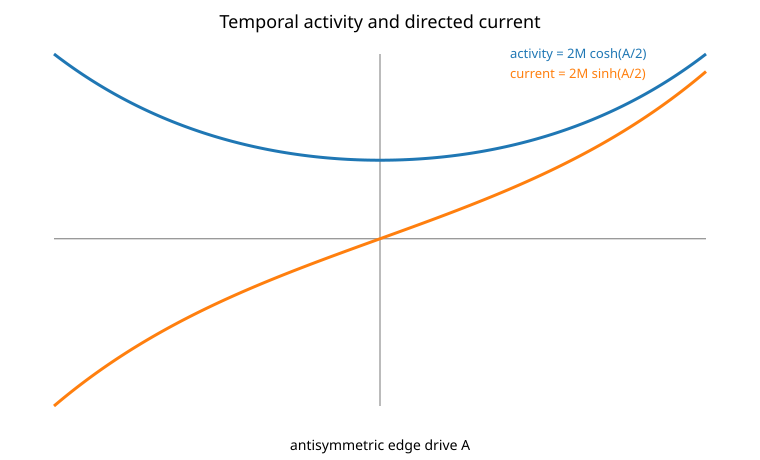
\includegraphics[width=0.86\textwidth]{figures/temporal_activity_decomposition.png}
\caption{Reference decomposition of one directed kinetic pair at fixed mobility $M=1$. Positive activity is even in the edge drive, while directed current is odd. The figure is generated by \texttt{scripts/build\_temporal\_activity\_figure.py}.}
\label{fig:temporal-activity-decomposition}
\end{figure}
